\documentclass{article}
\usepackage[UTF8]{ctex}
\usepackage[T1]{fontenc}
\usepackage[utf8]{inputenc}
\usepackage[colorlinks, linkcolor = black]{hyperref}
\usepackage{latexsym}
\usepackage{amsmath}
\usepackage{amssymb}
\usepackage{siunitx}
\usepackage{float}
\usepackage{algorithm}
\usepackage{algpseudocode}
\usepackage{xcolor}
\usepackage{geometry}
\usepackage{tikz}
\usepackage{subfigure}
\usetikzlibrary{positioning}
\usetikzlibrary[arrows, shapes, chains]
\makeatletter
\newenvironment{breakablealgorithm}
  {
   \begin{center}
     \refstepcounter{algorithm}% New algorithm
     \hrule height.8pt depth0pt \kern2pt% \@fs@pre for \@fs@ruled
     \renewcommand{\caption}[2][\relax]{% Make a new \caption
       {\raggedright\textbf{\textbf{算法}~\thealgorithm} ##2\par}%
       \ifx\relax##1\relax % #1 is \relax
         \addcontentsline{loa}{algorithm}{\protect\numberline{\thealgorithm}##2}%
       \else % #1 is not \relax
         \addcontentsline{loa}{algorithm}{\protect\numberline{\thealgorithm}##1}%
       \fi
       \kern2pt\hrule\kern2pt
     }
  }{
     \kern2pt\hrule\relax% \@fs@post for \@fs@ruled
   \end{center}
  }
\makeatother

\geometry{left = 3.5cm, right = 3.5cm}
\title{Homework 3}
\author{PB17000297 罗晏宸}
\date{April 13 2020}

\renewcommand{\algorithmicrequire}{\textbf{输入: }}
\renewcommand{\algorithmicensure}{\textbf{输出: }}
\renewcommand{\algorithmicindent}{2.0em}
\algdef{SE}{Begin}{End}{\textbf{Begin}}{\textbf{End}}
\algnewcommand\algorithmicparalleldo{\textbf{par-do}}
\algdef{S}[FOR]{ForAllinPar}[1]{\algorithmicforall\ #1\ \algorithmicparalleldo}
\algdef{S}[FOR]{ForinPar}[1]{\algorithmicfor\ #1\ \algorithmicparalleldo}
\floatname{algorithm}{\textbf{算法}}

\begin{document}
\maketitle

\section{Algorithm 10.1}
以下是上三角方程组回代解法的串行算法的形式化描述。
\begin{algorithm}[h]
    \caption{SISD 上回代求解上三角方程组算法}
    \begin{algorithmic}[1]
        \Require $\boldsymbol{A}_{n \times n}, \boldsymbol{b} = (b_1, \cdots, b_n)^\mathsf{T}$
        \Ensure $\boldsymbol{x} = (x_1, \cdots, x_n)^\mathsf{T}$
        \Begin
        \For{$i = n$ \textbf{downto} $1$}
        \State $x_i = b_i / a_{ii}$
        \For{$j = 1$ \textbf{to} $i - 1$} \label{j-loop}
        \State $b_j = b_j - a_{ji}x_i$
        \State $a_{ji} = 0$
        \EndFor
        \EndFor
        \End
    \end{algorithmic}
\end{algorithm}
\subparagraph{1} 请指出串行算法哪些部分可以并行化。
\subparagraph{2} 写出并行算法的形式化描述(需要注明计算模型类型),分析你的算法的时间复杂度

\paragraph{解}
\subparagraph{1}
算法第\ref{j-loop}行的$j$循环可以并行化。
\subparagraph{2}
在UMA模型上回代求解上三角方程组的并行算法如算法\ref{algorithm:UMA}所示。由\ref{i-loop}和\ref{P-loop}两行循环可知复杂度为$p(n) = p$,$t(n) = O(n)$
\begin{algorithm}[h]
    \caption{UMA 上回代求解上三角方程组算法}
    \label{algorithm:UMA}
    \begin{algorithmic}[1]
        \Require $\boldsymbol{A}_{n \times n}, \boldsymbol{b} = (b_1, \cdots, b_n)^\mathsf{T}$
        \Ensure $\boldsymbol{x} = (x_1, \cdots, x_n)^\mathsf{T}$
        \Begin
        \For{$i = n$ \textbf{downto} $1$} \label{i-loop}
        \State $x_i = b_i / a_{ii}$
        \ForAll{$P_j,\ 1 \leqslant j \leqslant p$} \label{P-loop}
        \For{$k = j$ \textbf{to} $i - 1$ \textbf{step} $p$} \Comment{$p$是处理器数}
        \State $b_k = b_k - a_{ki}x_i$
        \State $a_{ki} = 0$
        \EndFor
        \EndFor
        \EndFor
        \End
    \end{algorithmic}
\end{algorithm}

\section{Exercise 7.10}
顶点倒塌法是非常有名的求图的连通分量的算法,其基本思想是:连通的相邻的顶点可以合并成一个超顶点,并以它们中最小标号者标记之;此过程可继续在已合并的超顶点之间进行。在下列的算法中。$C(i)$表示与$i$相邻的最小的超顶点号码;$D(i)$表示顶点$i$所属连通分量的最小标号的顶点;$C(i) = \displaystyle \min_{j}{\{D(j) |_{A(i,j) = 1, D(i) \ne D(j)}\}}$语句为每个顶点$i$找与它不属于相同分量的相邻的最小号码的顶点$j$;语句$C(i) = \displaystyle \min_{j}{\{C(j) |_{D(j) = i, C(j) \ne i}\}}$表示把每个超顶点的根连到最小号码的相邻的超顶点的根上。 Hirschberg 的求连通分量算法如下。
\begin{breakablealgorithm}
    \caption{PRAM-CREW 上 Hirschberg 求连通分量算法}
    \label{algorithm:7.12}
    \begin{algorithmic}[1]
        \Require 邻接矩阵$\boldsymbol{A}_{n \times n}$
        \Ensure 向量 $\boldsymbol{D}(0 : n - 1)$,其中$D(i)$表示向量$\boldsymbol{D}$的分量
        \Begin
        \ForAllinPar{$i : 0 \leqslant i \leqslant n - 1$} \Comment{初始化 (1)}
        \State $D(i) = i$
        \EndFor
        \For{$\lceil \log{n} \rceil$ iterations} \label{BigLoop}
        \ForAllinPar{$i,j : 0 \leqslant i,j \leqslant n - 1$} \Comment{找相邻的最小者 (2)}
        \State $C(i) = \displaystyle \min_{j}{\{D(j) |_{A(i,j) = 1, D(i) \ne D(j)}\}}$
        \If{none} \State $C(i) = D(i)$ \EndIf
        \EndFor
        \ForAllinPar{$i,j : 0 \leqslant i,j \leqslant n - 1$} \Comment{找每个超顶点的最小相邻超顶点 (3)}
        \State $C(i) = \displaystyle \min_{j}{\{C(j) |_{D(j) = i, C(j) \ne i}\}}$
        \If{none} \State $C(i) = D(i)$ \EndIf
        \EndFor
        \ForAllinPar{$i : 0 \leqslant i \leqslant n - 1$} \Comment{ (4)}
        \State $D(i) = C(i)$
        \EndFor
        \For{$\lceil \log{n} \rceil$ iterations} \label{SmallLoop} \Comment{指针跳跃,找各顶点新的超顶点 (5)}
        \ForAllinPar{$i : 0 \leqslant i \leqslant n - 1$}
        \State $C(i) = C(C(i))$
        \EndFor
        \EndFor
        \ForAllinPar{$i : 0 \leqslant i \leqslant n - 1$} \Comment{ (6)}
        \State $D(i) = \min{\{C(i), D(C(i))\}}$
        \EndFor
        \EndFor
        \End
    \end{algorithmic}
\end{breakablealgorithm}

\subparagraph{(1)}试分析算法\ref{algorithm:7.12}的复杂度$t(n)$和$p(n)$。
\subparagraph{(2)}给定如图\ref{figure:7.11}所示无向图,试用算法\ref{algorithm:7.12}逐步求出该图的连通分量
\begin{figure}[h]
    \centering
    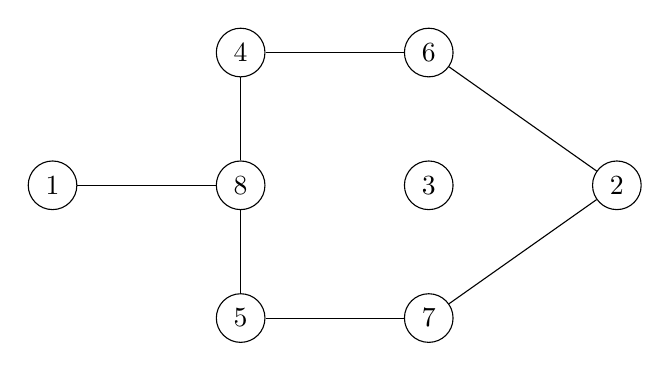
\begin{tikzpicture}
        \node[circle, draw] (1) {1};
        \node[circle, draw, right = 5.0em of 1] (8) {8};
        \node[circle, draw, right = 5.0em of 8] (3) {3};
        \node[circle, draw, right = 5.0em of 3] (2) {2};
        \node[circle, draw, above = 3.0em of 8] (4) {4};
        \node[circle, draw, above = 3.0em of 3] (6) {6};
        \node[circle, draw, below = 3.0em of 8] (5) {5};
        \node[circle, draw, below = 3.0em of 3] (7) {7};
        \draw[-] (1) -- (8);
        \draw[-] (4) -- (8);
        \draw[-] (5) -- (8);
        \draw[-] (4) -- (6);
        \draw[-] (5) -- (7);
        \draw[-] (2) -- (6);
        \draw[-] (2) -- (7);
    \end{tikzpicture}
    \\[2.0em]
    \begin{tabular}{c|cccccccccccc}
        顶点 &  &  & 1 & 2 & 3 & 4 & 5 & 6 & 7 & 8 &  & \\ \hline
        分量 &  &  & 1 & 2 & 3 & 4 & 5 & 6 & 7 & 8 &  &
    \end{tabular}
    \caption{待求连通分量的无向图}
    \label{figure:7.11}
\end{figure}

\paragraph{解}
\subparagraph{(1)}
注意到第\ref{BigLoop}行最外侧的循环迭代$\lceil \log{n} \rceil$次,在循环内第\ref{SmallLoop}行循环同样迭代$\lceil \log{n} \rceil$次,同时考虑外侧循环内的前两个Do in parallel循环语句中的求出最小值也是并行的,需要的处理器数为$(n - 1)^2$,因此算法的复杂度为$t(n) = O((\log{n})^2)$,$p(n) = O(n^2)$。

\subparagraph{(2)}
无向图共有8个结点,因此算法共进行$\lceil \log{8} \rceil = 3$次迭代,迭代过程如图\ref{figure:7.11Solution}所示。
% \begin{figure}[h]
%     \centering
%     \subfigure[初始化]{
%         \begin{tabular}{c|cccccccc}
%             顶点$i$ & 1 & 2 & 3 & 4 & 5 & 6 & 7 & 8 \\ \hline
%             $C(i)$  &   &   &   &   &   &   &   &   \\
%             $D(i)$  & 1 & 2 & 3 & 4 & 5 & 6 & 7 & 8
%         \end{tabular}
%     }
%     \quad
%     \subfigure[第一次迭代后的结果]{
%         \begin{tabular}{c|cccccccc}
%             顶点$i$ & 1 & 2 & 3 & 4 & 5 & 6 & 7 & 8 \\ \hline
%             $C(i)$  & 1 & 2 & 3 & 1 & 1 & 2 & 2 & 1 \\
%             $D(i)$  & 1 & 2 & 3 & 1 & 1 & 2 & 2 & 1
%         \end{tabular}
%     }

%     \subfigure[第二次迭代后的结果]{
%         \begin{tabular}{c|cccccccc}
%             顶点$i$ & 1 & 2 & 3 & 4 & 5 & 6 & 7 & 8 \\ \hline
%             $C(i)$  & 1 & 2 & 3 & 2 & 2 & 2 & 2 & 1 \\
%             $D(i)$  & 1 & 2 & 3 & 2 & 2 & 2 & 2 & 1
%         \end{tabular}
%     }
%     \quad
%     \subfigure[第三次迭代后的结果]{
%         \begin{tabular}{c|cccccccc}
%             顶点$i$ & 1 & 2 & 3 & 4 & 5 & 6 & 7 & 8 \\ \hline
%             $C(i)$  & 1 & 1 & 3 & 1 & 1 & 1 & 1 & 1 \\
%             $D(i)$  & 1 & 1 & 3 & 1 & 1 & 1 & 1 & 1
%         \end{tabular}
%     }
%     \caption{算法迭代过程}
%     \label{figure:7.11Solution}
% \end{figure}
\begin{figure}[h]
    \centering
    \begin{tabular}{c|c|cccccccc}
        迭代 & 顶点$i$ & 1 & 2 & 3 & 4 & 5 & 6 & 7 & 8 \\ \hline
        (1) & $D(i)$  & 1 & 2 & 3 & 4 & 5 & 6 & 7 & 8 \\ \hline
        (2) & $C(i)$  & 8 & 6 & 3 & 6 & 7 & 2 & 2 & 1 \\
        (3) & $C(i)$  & 8 & 6 & 3 & 6 & 7 & 2 & 2 & 1 \\
        (4) & $D(i)$  & 8 & 6 & 3 & 6 & 7 & 2 & 2 & 1 \\
        (5) & $C(i)$  & 1 & 2 & 3 & 2 & 2 & 6 & 6 & 8 \\
        (6) & $D(i)$  & 1 & 2 & 3 & 2 & 2 & 2 & 2 & 1 \\ \hline
        (2) & $C(i)$  & 1 & 2 & 3 & 1 & 1 & 2 & 2 & 2 \\
        (3) & $C(i)$  & 2 & 1 & 3 & 2 & 2 & 2 & 2 & 1 \\
        (4) & $D(i)$  & 2 & 1 & 3 & 2 & 2 & 2 & 2 & 1 \\
        (5) & $C(i)$  & 1 & 2 & 3 & 1 & 1 & 1 & 1 & 2 \\
        (6) & $D(i)$  & 1 & 1 & 3 & 1 & 1 & 1 & 1 & 1 \\ \hline
        (2) & $C(i)$  & 1 & 1 & 3 & 1 & 1 & 1 & 1 & 1 \\
        (3) & $C(i)$  & 1 & 1 & 3 & 1 & 1 & 1 & 1 & 1 \\
        (4) & $D(i)$  & 1 & 1 & 3 & 1 & 1 & 1 & 1 & 1 \\
        (5) & $C(i)$  & 1 & 1 & 3 & 1 & 1 & 1 & 1 & 1 \\
        (6) & $D(i)$  & 1 & 1 & 3 & 1 & 1 & 1 & 1 & 1
    \end{tabular}
    \caption{算法迭代过程}
    \label{figure:7.11Solution}
\end{figure}
\end{document}